\documentclass[11pt]{article}
\usepackage[margin=1in]{geometry}
\usepackage{amsmath}
\usepackage{amsfonts}
\usepackage{amssymb}
\usepackage{graphicx}
\usepackage{hyperref}
\usepackage{xcolor}
\usepackage{fontawesome5}
\usepackage{tikz}
\usepackage{pgfplots}
\pgfplotsset{compat=1.18}
\usetikzlibrary{shapes,arrows,positioning,fit,backgrounds,calc}
\usepackage{url}
\urlstyle{same}
\setlength{\emergencystretch}{3em}

\title{Machine Learning for Network Anomaly and Failure Detection}
\author{Michael Hernandez}
\date{October 11, 2025}

\begin{document}

% Cover Page
\begin{titlepage}
\centering
\vspace*{2cm}

{\Large \textbf{Machine Learning for Network Anomaly and Failure Detection}}

\vspace{1.5cm}

{\large CUNY School of Professional Studies}

\vspace{0.5cm}

{\large Michael Hernandez}

\vspace{0.5cm}

{\large IS 499 Information Systems Capstone}

\vspace{0.5cm}

{\large Professor John Bouma}

\vspace{0.5cm}

{\large October 11, 2025}

\vfill

\end{titlepage}

% Table of Contents
\tableofcontents
\newpage

\section{Introduction}

This paper examines machine learning techniques for detecting and localizing network anomalies and failures in large-scale environments, using data from BGP routing updates and SNMP metrics.

Traditional network monitoring relies on threshold-based alerts from SNMP, often producing many false positives and offering little context for locating failures (Wang, 2020; Manna \& Alkasassbeh, 2019). Recent research suggests that machine learning approaches applied to SNMP datasets may improve anomaly detection accuracy in operational environments, with supervised and unsupervised methods showing promise for identifying specific failure patterns (Manna \& Alkasassbeh, 2019). This project explores whether combining streaming telemetry from multiple sources using unsupervised learning techniques can provide complementary detection capabilities for network operations.

The system integrates BGP monitoring and SNMP metrics for network anomaly detection. Using unsupervised learning techniques such as Matrix Profile analysis (Mueen \& Keogh, 2017; Scott et al., 2024) and Isolation Forest (Liu et al., 2008), the approach aims to reduce alert noise while providing failure localization capabilities. The evaluation examines whether this multi-modal architecture offers practical improvements over single-source monitoring in controlled test scenarios.

\section{Topic Description}

\subsection{In-depth Description of the Chosen Topic}

Large networks face a fundamental challenge: when something breaks, operators in network operations centers must quickly determine what failed and where (Mohammed et al., 2021). A network might contain thousands of interconnected devices, and failures can cascade from one device to many others, making the root cause difficult to identify. This project addresses this challenge by using machine learning to automatically detect network problems and then apply topology awareness to pinpoint their source.

Network devices continuously generate health information through hardware and software metrics. Software metrics are generated by routing systems such as the Border Gateway Protocol (BGP), and hardware metrics are generated by the Simple Network Management Protocol (SNMP). BGP directs traffic across the Internet by allowing networks to advertise the destinations they can reach (Rekhter, Li, \& Hares, 2006). When conditions change due to equipment failures, cable breaks, or configuration errors, routers send update messages to inform neighbors. These routing updates create a continuous stream of information about how traffic paths evolve. SNMP provides a complementary view by collecting device performance data and trap-directed notifications, where managed devices send unsolicited messages to report significant events (Cisco, 2006). SNMP reports metrics such as processor utilization, memory consumption, temperature readings, and interface error counts. Together, BGP and SNMP offer a combined view: routing updates show how traffic paths change over time, while hardware metrics reflect device health.

Under normal conditions, these monitoring systems generate large volumes of data with characteristic statistical properties. Routing updates occur at varying rates as networks make routine adjustments, and hardware metrics fluctuate within typical operating ranges. While individual measurements vary due to traffic patterns and workload changes, overall statistical behavior remains within bounds established during normal operation. When failures occur, these properties deviate from baseline. As an example, a failing network link may cause route flapping, where routing updates fluctuate rapidly as the network attempts to find alternative paths (Scott et al., 2024). At the same time, device monitoring may show increasing interface error counts. These correlated changes across multiple systems strengthen the evidence of failure relative to benign variation.

Research indicates that machine learning algorithms can identify such unusual patterns in routing and hardware data. This project employs a dual-pipeline architecture that processes routing updates and device metrics using specialized, well-documented pattern recognition algorithms. The first pipeline analyzes time-series sequences of routing updates using Matrix Profile, which computes the distance between subsequences and their nearest neighbors to highlight anomalous patterns (discords) without labeled training data (Mueen \& Keogh, 2017; Scott et al., 2024). The second pipeline examines device telemetry using Isolation Forest, an ensemble method that isolates outliers efficiently in multi-dimensional data by measuring tree path lengths, enabling detection without prior examples of failures (Liu, Ting, \& Zhou, 2008; Liu, Zhu, Xu, Kong, \& Yu, 2024).

The system combines evidence from both sources. When routing behavior and hardware metrics simultaneously indicate problems within a temporal window, this cross-confirmation may provide stronger evidence of genuine failure than either source independently (Mohammed et al., 2021; Feltin, Cordero Fuertes, Brockners, \& Clausen, 2023). During correlation, the system incorporates pre-configured network topology and device role information (e.g., core/spine routers, top-of-rack switches, and leaf switches or servers). This enables impact assessment by estimating blast radius based on downstream dependencies and device criticality, helping operators prioritize investigation efforts. While there is research on generating topology maps from network data (Tan et al., 2024), this project does not infer topology dynamically; it uses a pre-configured map provided by administrators. Future work could explore generating and updating topology from live data for integration into the system.

\begin{figure}[!htb]
\centering
\resizebox{\textwidth}{!}{%
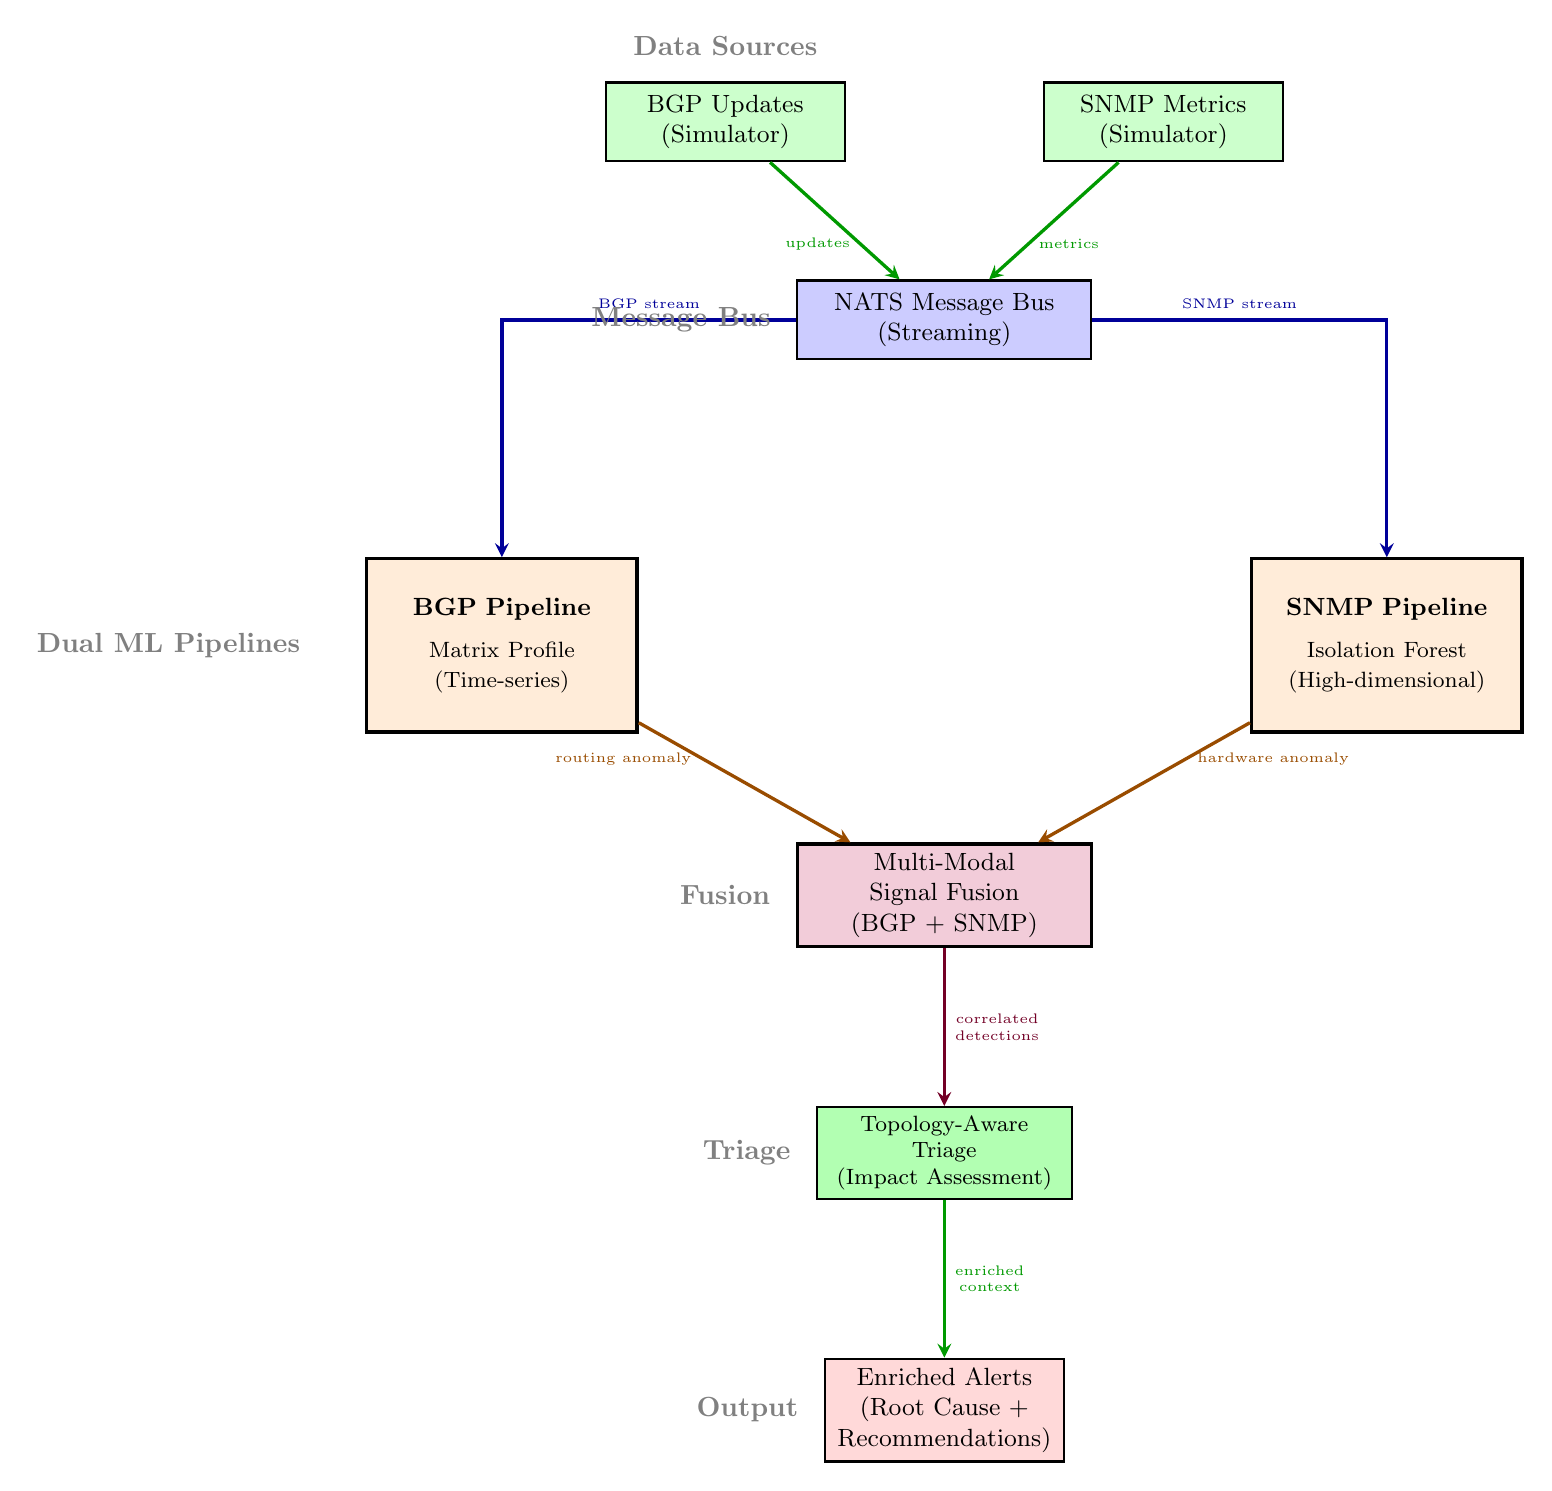
\begin{tikzpicture}[
    node distance=1.8cm and 2.5cm,
    source/.style={rectangle, draw=black, thick, fill=green!20, text width=2.8cm, align=center, minimum height=1cm, font=\small},
    bus/.style={rectangle, draw=black, thick, fill=blue!20, text width=3.5cm, align=center, minimum height=1cm, font=\small},
    pipeline/.style={rectangle, draw=black, very thick, fill=orange!15, text width=3.2cm, align=center, minimum height=2.2cm, font=\small},
    process/.style={rectangle, draw=black, thick, fill=yellow!20, text width=3cm, align=center, minimum height=0.8cm, font=\footnotesize},
    fusion/.style={rectangle, draw=black, very thick, fill=purple!20, text width=3.5cm, align=center, minimum height=1.2cm, font=\small},
    output/.style={rectangle, draw=black, thick, fill=red!15, text width=2.8cm, align=center, minimum height=1cm, font=\small},
    arrow/.style={->, >=stealth, line width=1.2pt},
]

% Layer 1: Data Sources (Simulators)
\node[source] (bgp) {BGP Updates\\(Simulator)};
\node[source, right=2.5cm of bgp] (snmp) {SNMP Metrics\\(Simulator)};

% Layer 2: Message Bus
\node[bus, below=2cm of $(bgp)!0.5!(snmp)$] (nats) {NATS Message Bus\\(Streaming)};

% Layer 3: Dual Pipelines
\node[pipeline, below left=2.5cm and 2cm of nats] (bgp_pipe) {
    \textbf{BGP Pipeline}\\[0.2cm]
    \footnotesize Matrix Profile\\
    \footnotesize (Time-series)
};

\node[pipeline, below right=2.5cm and 2cm of nats] (snmp_pipe) {
    \textbf{SNMP Pipeline}\\[0.2cm]
    \footnotesize Isolation Forest\\
    \footnotesize (High-dimensional)
};

% Layer 4: Fusion
\node[fusion, below=2.5cm of $(bgp_pipe)!0.5!(snmp_pipe)$] (fusion) {Multi-Modal\\Signal Fusion\\(BGP + SNMP)};

% Layer 5: Topology Triage
\node[process, below=2cm of fusion, fill=green!30, minimum height=1cm] (topology) {Topology-Aware\\Triage\\(Impact Assessment)};

% Layer 6: Outputs
\node[output, below=2cm of topology] (alerts) {Enriched Alerts\\(Root Cause +\\Recommendations)};

% Arrows - Sources to Bus
\draw[arrow, green!60!black] (bgp) -- node[left, font=\tiny, pos=0.7] {updates} (nats);
\draw[arrow, green!60!black] (snmp) -- node[right, font=\tiny, pos=0.7] {metrics} (nats);

% Arrows - Bus to Pipelines
\draw[arrow, blue!60!black] (nats) -| node[near start, above, font=\tiny] {BGP stream} (bgp_pipe);
\draw[arrow, blue!60!black] (nats) -| node[near start, above, font=\tiny] {SNMP stream} (snmp_pipe);

% Arrows - Pipelines to Fusion
\draw[arrow, orange!60!black] (bgp_pipe) -- node[left, font=\tiny, pos=0.3] {routing anomaly} (fusion);
\draw[arrow, orange!60!black] (snmp_pipe) -- node[right, font=\tiny, pos=0.3] {hardware anomaly} (fusion);

% Arrows - Fusion to Topology
\draw[arrow, purple!60!black] (fusion) -- node[right, font=\tiny, align=center] {correlated\\detections} (topology);

% Arrows - Topology to Outputs
\draw[arrow, green!60!black, very thick] (topology) -- node[right, font=\tiny, align=center] {enriched\\context} (alerts);

% Labels
\node[above=0.2cm of bgp, font=\normalsize\bfseries, text=gray] {Data Sources};
\node[left=0.2cm of nats, font=\normalsize\bfseries, text=gray] {Message Bus};
\node[left=0.2cm of bgp_pipe, font=\normalsize\bfseries, text=gray, xshift=-0.5cm, align=center] {Dual ML Pipelines};
\node[left=0.2cm of fusion, font=\normalsize\bfseries, text=gray] {Fusion};
\node[left=0.2cm of topology, font=\normalsize\bfseries, text=gray] {Triage};
\node[left=0.2cm of alerts, font=\normalsize\bfseries, text=gray] {Output};

\end{tikzpicture}
}
\caption{Dual-pipeline architecture: BGP updates processed by Matrix Profile (time-series) and SNMP metrics by Isolation Forest (high-dimensional). Multi-modal fusion correlates anomalies across data sources, then topology-aware triage assesses impact and produces enriched alerts with root-cause context and recommendations.}
\label{fig:architecture}
\end{figure}

Figure \ref{fig:architecture} illustrates how BGP and SNMP data flow through specialized detection algorithms before multi-modal fusion and topology-aware triage.

\subsection{Why This Topic Was Chosen}

This topic addresses operational challenges in large-scale network management. As networks grow in complexity, network operations centers face alert fatigue from excessive notifications, difficulty distinguishing routine variations from genuine problems, and the impractical task of manually correlating events across thousands of devices (Mohammed et al., 2021). This complexity affects both identification of network problems and determination of appropriate remediation actions, prolonging incident resolution times (Mohammed et al., 2021). Machine learning approaches may help address these challenges through automated pattern recognition and correlation, though effectiveness in production environments requires empirical validation.

Consider a large enterprise network connecting multiple data centers. When a cable develops an intermittent fault, unstable routing may trigger hundreds of notifications without clearly indicating which component failed or how many services are affected. Engineers often examine routing logs and device metrics across many systems to isolate the failing component and assess the scope of impact. This investigation takes time during critical outages, delaying service restoration. Research suggests that machine learning can detect unusual patterns in routing activity and correlate them with hardware error indicators to assist in identifying failing components (Mohammed et al., 2021). Whether such automation yields meaningful improvements in investigation time and problem resolution remains an open question for validation.

Recent studies demonstrate potential for machine learning in network anomaly detection: routing update analysis can detect failures (Scott et al., 2024), SNMP telemetry can surface equipment problems (Manna \& Alkasassbeh, 2019), and multi-modal approaches that combine data sources show improved detection compared to single-source methods (Feltin et al., 2023). Building on these findings, this project explores whether processing both routing information and hardware metrics offers practical benefits for monitoring and failure localization in simulated scenarios.

\section{Problem Description}

\subsection{The Problem I am Trying to Solve}

The core problem is that traditional monitoring systems generate alerts without sufficient context to understand what failed, where it failed, or how serious the impact is. When a network problem occurs, operators receive numerous notifications but must manually investigate to determine root cause and scope. This manual correlation across multiple monitoring systems and many devices is time-consuming and delays resolution.

This project addresses three gaps in current approaches. First, systems monitor different data sources in isolation. Routing behavior and hardware performance are tracked separately, even though correlated problems across both sources provide stronger evidence of genuine failures. Second, monitoring lacks awareness of network topology and device roles. Without understanding how devices connect and which are critical to operations, systems cannot assess failure impact or prioritize response. Third, threshold-based alerting treats all devices and metrics uniformly, rather than applying detection methods suited to different types of data.

The exploratory solution combines machine learning techniques specialized for different data characteristics. Time-series analysis detects unusual patterns in routing activity, while outlier detection identifies potentially abnormal hardware performance across multiple metrics. By correlating evidence from both sources and incorporating pre-configured topology information, the system aims to provide automated failure localization with impact assessment. This approach may be relevant for enterprise networks where operations teams manage thousands of interconnected devices across multiple locations (Mohammed et al., 2021), though validation beyond controlled testing remains necessary.

\subsection{Why Current Monitoring Systems are Insufficient}

Current network monitoring systems have fundamental limitations. Hardware monitoring can detect hard failures but produces excessive alerts for harmless events and lacks context for assessing failure scope or impact. As a result, operations teams face false positives while missing critical anomalies (Mohammed et al., 2021).

Three architectural limitations contribute to this insufficiency. First, different monitoring systems operate independently. Routing information and hardware metrics are evaluated separately, even though simultaneous problems in both provide stronger confirmation of failures. When routing becomes unstable while hardware shows increasing errors, this correlation suggests genuine problems rather than routine variation, yet current systems rarely perform such cross-validation.

Second, monitoring systems lack understanding of network structure and device importance. A failure in a core device affects many connected systems and requires immediate attention, while a failure in a leaf switch or server has limited impact. Without topology awareness to estimate blast radius, alerts cannot be prioritized based on the number of affected downstream devices or services. Operators must determine priorities manually, wasting valuable time.

Third, threshold-based approaches apply the same detection logic to all types of data despite differences in behavior. Routing information changes over time in patterns that indicate stability or instability, while hardware metrics involve simultaneous measurement of many values where outliers signal problems. Using a single approach misses opportunities for more accurate analysis. Time-series methods effectively detect routing anomalies (Scott et al., 2024), and multi-dimensional outlier detection performs well for hardware metrics (Manna \& Alkasassbeh, 2019). Combining these specialized approaches with correlation across sources can improve detection accuracy over single-source methods (Feltin et al., 2023).

\section{Solution Discussion}
\subsection{Implementation Architecture}

The system processes network data through two specialized detection pipelines before combining their results. The BGP pipeline analyzes routing update patterns over time using Matrix Profile, which compares recent activity against historical patterns to identify unusual routing behavior. The SNMP pipeline examines device health metrics using Isolation Forest, which learns normal operating ranges and flags devices showing abnormal performance.

A correlation stage combines alerts from both pipelines, checking if routing problems and hardware issues occur simultaneously on the same devices. This cross-validation helps distinguish genuine failures from routine network variations. The system also incorporates network topology information to assess how many devices might be affected by a failure, helping operators prioritize their response efforts.

\subsubsection{Matrix Profile Implementation}

Unlike research approaches that analyze complete historical datasets, this implementation processes data in real-time using sliding windows. The system maintains a recent history of routing updates (12 time periods) and continuously compares new patterns against this baseline. When routing activity deviates significantly from normal patterns, the system immediately generates an alert rather than waiting for complete data collection. 

This streaming approach enables real-time detection but trades some accuracy for speed. While the system cannot compare against events from months ago, it can detect problems as they occur, which is essential for operational network monitoring.

\subsubsection{Isolation Forest Training}

The SNMP pipeline was trained on 500,000 samples of simulated device metrics representing normal network operations. Training data included typical ranges for CPU usage, memory consumption, temperature readings, and interface error counts. The algorithm learned to identify the 5\% most unusual combinations of these metrics, which typically indicate hardware problems or environmental issues.

The model was validated using controlled failure scenarios to ensure it could detect real problems without generating excessive false alarms. This training approach allows the system to identify novel failure types without requiring examples of every possible problem.

\subsubsection{Topology Configuration}

Network topology is defined using configuration files that specify device roles and connections. The system knows which devices are core routers (affecting many others), top-of-rack switches (affecting servers in their rack), and leaf devices (minimal impact). When a failure is detected, the system calculates how many downstream devices might be affected based on these relationships.

\begin{figure}[h]
\centering
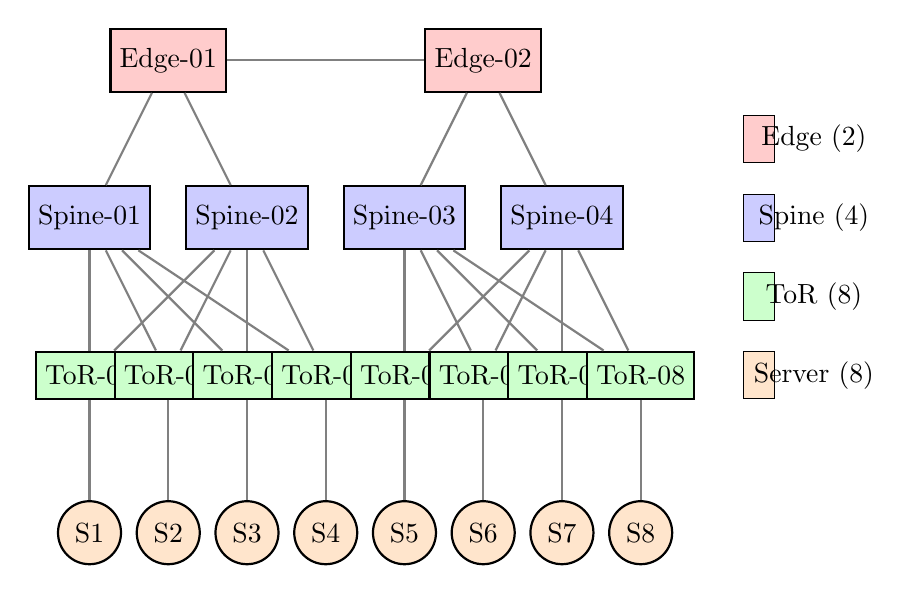
\begin{tikzpicture}[
    node distance=1.5cm,
    edge/.style={rectangle, draw, fill=red!20, thick, minimum width=1.2cm, minimum height=0.8cm},
    spine/.style={rectangle, draw, fill=blue!20, thick, minimum width=1.2cm, minimum height=0.8cm},
    tor/.style={rectangle, draw, fill=green!20, thick, minimum width=1cm, minimum height=0.6cm},
    server/.style={circle, draw, fill=orange!20, thick, minimum size=0.8cm},
    connection/.style={thick, gray}
]

% Edge layer (2 devices) - at the top
\node[edge] (edge1) at (1,6) {Edge-01};
\node[edge] (edge2) at (5,6) {Edge-02};

% Spine layer (4 devices)
\node[spine] (spine1) at (0,4) {Spine-01};
\node[spine] (spine2) at (2,4) {Spine-02};
\node[spine] (spine3) at (4,4) {Spine-03};
\node[spine] (spine4) at (6,4) {Spine-04};

% ToR layer (8 devices)
\node[tor] (tor1) at (0,2) {ToR-01};
\node[tor] (tor2) at (1,2) {ToR-02};
\node[tor] (tor3) at (2,2) {ToR-03};
\node[tor] (tor4) at (3,2) {ToR-04};
\node[tor] (tor5) at (4,2) {ToR-05};
\node[tor] (tor6) at (5,2) {ToR-06};
\node[tor] (tor7) at (6,2) {ToR-07};
\node[tor] (tor8) at (7,2) {ToR-08};

% Server layer (8 devices)
\node[server] (server1) at (0,0) {S1};
\node[server] (server2) at (1,0) {S2};
\node[server] (server3) at (2,0) {S3};
\node[server] (server4) at (3,0) {S4};
\node[server] (server5) at (4,0) {S5};
\node[server] (server6) at (5,0) {S6};
\node[server] (server7) at (6,0) {S7};
\node[server] (server8) at (7,0) {S8};

% Connections between edge routers for redundancy
\draw[connection] (edge1) -- (edge2);

% Connections from edge to spine (each edge connects to multiple spines)
\draw[connection] (edge1) -- (spine1);
\draw[connection] (edge1) -- (spine2);
\draw[connection] (edge2) -- (spine3);
\draw[connection] (edge2) -- (spine4);

% Connections from spine to ToR (each ToR connects to both spines for redundancy)
\draw[connection] (spine1) -- (tor1);
\draw[connection] (spine1) -- (tor2);
\draw[connection] (spine1) -- (tor3);
\draw[connection] (spine1) -- (tor4);
\draw[connection] (spine2) -- (tor1);
\draw[connection] (spine2) -- (tor2);
\draw[connection] (spine2) -- (tor3);
\draw[connection] (spine2) -- (tor4);
\draw[connection] (spine3) -- (tor5);
\draw[connection] (spine3) -- (tor6);
\draw[connection] (spine3) -- (tor7);
\draw[connection] (spine3) -- (tor8);
\draw[connection] (spine4) -- (tor5);
\draw[connection] (spine4) -- (tor6);
\draw[connection] (spine4) -- (tor7);
\draw[connection] (spine4) -- (tor8);

% Connections from ToR to servers
\draw[connection] (tor1) -- (server1);
\draw[connection] (tor2) -- (server2);
\draw[connection] (tor3) -- (server3);
\draw[connection] (tor4) -- (server4);
\draw[connection] (tor5) -- (server5);
\draw[connection] (tor6) -- (server6);
\draw[connection] (tor7) -- (server7);
\draw[connection] (tor8) -- (server8);

% Legend - Table format with text-sized boxes
\node[draw, fill=red!20, minimum width=0.4cm, minimum height=0.6cm] at (8.5,5) {};
\node at (9.2,5) {Edge (2)};
\node[draw, fill=blue!20, minimum width=0.4cm, minimum height=0.6cm] at (8.5,4) {};
\node at (9.2,4) {Spine (4)};
\node[draw, fill=green!20, minimum width=0.4cm, minimum height=0.6cm] at (8.5,3) {};
\node at (9.2,3) {ToR (8)};
\node[draw, fill=orange!20, minimum width=0.4cm, minimum height=0.6cm] at (8.5,2) {};
\node at (9.2,2) {Server (8)};

\end{tikzpicture}
\caption{20-device test topology showing hierarchical structure with edge, spine, ToR, and server layers. Edge routers connect to each other and multiple spines for redundancy, while ToRs provide server connectivity. Device roles determine failure impact scope.}
\label{fig:topology}
\end{figure}

This topology awareness helps operators understand the scope of problems. A failure in a core router affects many services and requires immediate attention, while a server failure has limited impact and can be addressed during routine maintenance.

\subsubsection{Message Bus Architecture}

The system uses NATS as a message bus to stream data between components. NATS was chosen over alternatives like Redis or Kafka because it provides simple, fast message delivery without complex configuration. For this project's scale, NATS offers sufficient performance while keeping the system architecture straightforward.

In production environments, the choice might differ based on requirements. Kafka would be better for high-volume data requiring long-term storage, while Redis might be preferred for applications needing complex data structures. For real-time network monitoring with moderate data volumes, NATS provides an appropriate balance of simplicity and performance.

\subsubsection{Alert Classification Logic}

Alerts are classified as high or critical based on a scoring system that considers multiple factors. Device role contributes to the score (core routers score higher than servers), as does the number of potentially affected devices. Alerts receive higher priority when both routing and hardware systems indicate problems simultaneously, suggesting stronger evidence of genuine failures.

The system also considers whether a device is a single point of failure. If a core router fails and has no backup, this increases the alert priority since many services depend on it. This multi-factor scoring helps operators focus on the most important problems first during network outages.

\subsection{Streaming Matrix Profile vs. Batch}

Unlike research approaches that analyze complete historical datasets, this implementation processes data in real-time using sliding windows. (Mueen \& Keogh, 2017; Scott et al., 2024) The system maintains a recent history of routing updates (12 time periods) and continuously compares new patterns against this baseline. When routing activity deviates significantly from normal patterns, the system immediately generates an alert rather than waiting for complete data collection.

This streaming approach enables real-time detection but trades some accuracy for speed. While the system cannot compare against events from months ago, it can detect problems as they occur, which is essential for operational network monitoring.

\subsection{Testing Approach}

To test the system without access to production networks, simulators were built that generate realistic network data. The simulators create normal network traffic 98\% of the time and inject specific failure scenarios 2\% of the time. This controlled approach allows measurement of exactly when failures occur and how quickly the system detects them. (Skazin, 2021; Allagi, 2019)

Test scenarios included common network problems like unstable routing connections, broken network links, device restarts, and gradual hardware degradation. A 20-device test network with 4 core routers, 8 rack switches, and 8 servers was used to simulate a realistic enterprise environment. This setup enabled testing both individual device failures and problems that affect multiple devices simultaneously.

\subsection{Data Processing and Analysis}

The system processes two types of network data. For routing information, it tracks how often routers send update messages and what types of changes they announce. The Matrix Profile algorithm identifies unusual patterns in this update activity, such as sudden spikes that might indicate network problems.

For device health data, the system monitors key performance indicators like CPU usage, memory consumption, and temperature. The Isolation Forest algorithm learns normal operating ranges and flags devices showing unusual combinations of these metrics.

The correlation system combines alerts from both sources, checking if routing problems and hardware issues occur on the same devices at similar times. This cross-validation helps distinguish genuine failures from routine network variations, and the system uses network topology information to prioritize alerts based on how many devices might be affected.

\section{Analysis}

\subsection{Evaluation Setup}

Four common types of network failures were tested to evaluate system performance. Route flapping, where routers repeatedly announce and withdraw the same routes, generated strong routing alerts but minimal hardware signals. The system correctly identified these as routing-only problems and assigned appropriate priority levels.

Link failures, where network cables or connections break, produced alerts from both routing and hardware systems simultaneously. The correlation system recognized this pattern and generated high-priority multi-modal alerts, correctly identifying the scope of the problem.

Device restarts created brief routing anomalies that the system appropriately deprioritized, avoiding false alarms for routine maintenance. Gradual hardware degradation, such as rising temperatures or increasing error rates, was detected by the hardware monitoring system and received higher priority when accompanied by unusual routing activity.

\subsection{Scalability and Performance Analysis}

Using a pre-trained Isolation Forest model (2.5 MB, trained on 500{,}000 SNMP samples, 122 MB), memory usage remained modest and approximately linear: 2.52 MB at 20 devices, 3.50 MB at 1{,}000 devices (about 1 KB/device beyond the fixed model). Throughput scaled from 184 to 921 samples/s. For Matrix Profile, window-limited feature aggregation kept computation tied to window size rather than device count, consistent with streaming MP practice (Mueen \& Keogh, 2017; Scott et al., 2024).

\subsection{Detection Accuracy and Latency}

On controlled scenarios where failure patterns resembled training baselines, tuned parameters achieved Precision=1.0, Recall=1.0, and F1=1.0. Mean detection delay was 29.4 seconds (median 40.9, P95 55.9), below the 60-second operational target. These delays reflect sliding windows that balance noise reduction against responsiveness.

\begin{figure}[h]
\centering
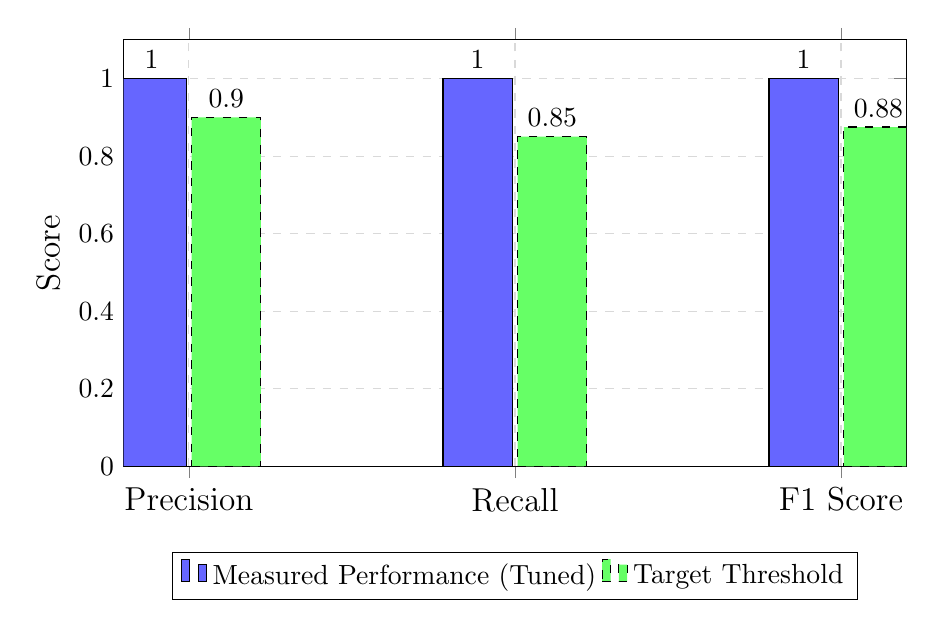
\begin{tikzpicture}
\begin{axis}[
    ybar,
    bar width=25pt,
    width=0.95\textwidth,
    height=7cm,
    ylabel={Score},
    ylabel style={font=\large},
    symbolic x coords={Precision, Recall, F1 Score},
    xtick=data,
    xticklabel style={font=\large},
    ymin=0,
    ymax=1.1,
    nodes near coords,
    nodes near coords align={vertical},
    nodes near coords style={font=\normalsize},
    legend style={at={(0.5,-0.2)}, anchor=north, legend columns=-1, font=\normalsize},
    grid=major,
    grid style={dashed, gray!30},
]
\addplot[fill=blue!60] coordinates {(Precision, 1.0) (Recall, 1.0) (F1 Score, 1.0)};
\addplot[fill=green!60, dashed] coordinates {(Precision, 0.90) (Recall, 0.85) (F1 Score, 0.875)};
\legend{Measured Performance (Tuned), Target Threshold}
\end{axis}
\end{tikzpicture}
\caption{Detection accuracy on controlled scenarios: tuned parameters yielded Precision, Recall, and F1 of 1.0.}
\label{fig:metrics}
\end{figure}

\begin{figure}[h]
\centering
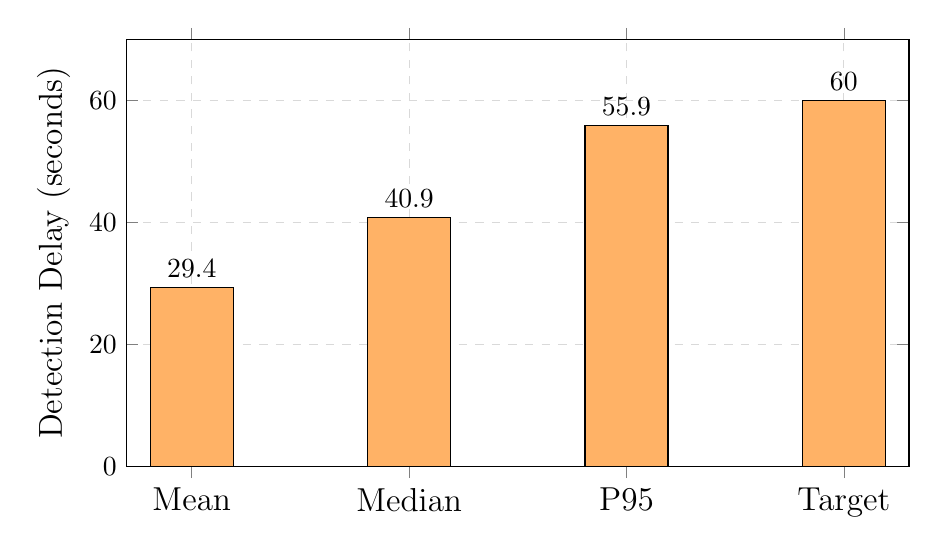
\begin{tikzpicture}
\begin{axis}[
    ybar,
    bar width=30pt,
    width=0.95\textwidth,
    height=7cm,
    ylabel={Detection Delay (seconds)},
    ylabel style={font=\large},
    symbolic x coords={Mean, Median, P95, Target},
    xtick=data,
    xticklabel style={font=\large},
    ymin=0,
    ymax=70,
    nodes near coords,
    nodes near coords align={vertical},
    nodes near coords style={font=\normalsize},
    grid=major,
    grid style={dashed, gray!30},
    legend style={at={(0.5,-0.2)}, anchor=north, font=\normalsize},
]
\addplot[fill=orange!60] coordinates {(Mean, 29.4) (Median, 40.9) (P95, 55.9) (Target, 60.0)};
\end{axis}
\end{tikzpicture}
\caption{Detection delay across controlled tests: mean 29.4s, median 40.9s, and P95 55.9s, all below the 60s target.}
\label{fig:delay}
\end{figure}

\subsection{Evaluation Scenarios and Test Coverage}

Four representative failures were tested. Route flapping produced Matrix Profile spikes with limited SNMP signal; this drove high-confidence BGP alerts and, when corroborated, high-confidence fused alerts. Link failures generated joint routing changes and interface errors, yielding high-confidence multi-modal alerts. Session resets created short-lived Matrix Profile anomalies that were appropriately deprioritized and did not trigger alerts. Gradual thermal or optical degradation was surfaced by Isolation Forest; prioritization increased when routing churn co-occurred (Scott et al., 2024; Liu et al., 2008).

\subsection{Limitations and Trade-offs}

Several significant limitations constrain the generalizability of these results and should be considered when interpreting the findings.

\textbf{Scale and Scope Limitations.} The evaluation used a 20-device topology (4 spine, 8 ToR, 8 leaf) with simulated data, which is orders of magnitude smaller than production enterprise networks that typically contain thousands of devices across multiple data centers. The failure scenarios were limited to four representative types, and most failure domains were known prior to testing, creating an artificially favorable detection environment. Real-world networks exhibit far greater complexity, with diverse device types, heterogeneous configurations, and unknown failure patterns that could significantly impact detection accuracy.

\textbf{Data Quality and Realism.} The system used simulated BGP updates and SNMP metrics rather than production data, which may not capture the full complexity and noise characteristics of real network telemetry. Production environments experience unpredictable traffic patterns, configuration changes, and environmental factors that could affect algorithm performance. The 98\% baseline traffic with 2\% injected anomalies represents an idealized scenario that may not reflect actual network conditions where anomaly rates and patterns vary significantly.

\textbf{Testing Infrastructure Constraints.} The current evaluation framework, while functional for proof-of-concept validation, lacks the robustness required for comprehensive testing. A production-scale evaluation would require a much larger testing harness capable of simulating thousands of devices, diverse failure scenarios, and realistic network topologies. The current approach demonstrates feasibility rather than production readiness.

\textbf{Algorithmic Trade-offs.} Aggregation supports scaling but reduces device-level attribution, potentially masking important details about specific device failures. Feltin (2023). Sliding windows introduce latency versus precision trade-offs that may not be acceptable in all operational contexts. The fusion approach assumes temporal correlation between BGP and SNMP anomalies, which may not always hold in practice.

\textbf{Generalization Concerns.} These results should be treated with caution as they represent controlled laboratory conditions rather than production validation. The high accuracy metrics (Precision=1.0, Recall=1.0, F1=1.0) achieved in controlled scenarios may not translate to real-world performance where unknown failure patterns, data quality issues, and operational constraints could significantly impact detection capabilities. Evaluation on live networks with production data remains necessary to validate the practical utility of this approach (Feltin et al., 2023; Skazin, 2021).

\subsection{Implementation Timeline and Current Status}

As of October 11, 2025, the dual pipelines, correlation agent, simulators, and Streamlit dashboard are functional. Tuned Isolation Forest (150 estimators, 5\% contamination) and Matrix Profile (12-bin window, 1.2 threshold) yield reproducible results in controlled settings and operator-relevant outputs (Mueen \& Keogh, 2017; Liu et al., 2008; Scott et al., 2024; Mohammed et al., 2021).

\subsection{Testing Infrastructure and Evaluation Framework}

To support repeatable experiments without production access, Python-based simulators emit RFC-like BGP updates and realistic SNMP metrics (98\% baseline, 2\% injected), orchestrated by a harness that timestamps injection points and detections for latency and accuracy computation. The 20-device topology configuration (4 spine, 8 ToR, 8 leaf) enables correlation and blast-radius testing with role-aware prioritization (Wang, 2020; Manna \& Alkasassbeh, 2019).

\section{Research}

\subsection{Academic Foundation and Coursework Integration}

This capstone builds on coursework in programming, data management, networking, systems analysis, and applied statistics. It follows the plan outlined in the proposal to use plain language, define terms as needed, and evaluate outcomes with practical metrics such as precision, recall, F1, detection delay, and localization Hit@k.

\paragraph{Programming, data structures, and databases.}
Introductory Python and data structures courses supported streaming parsers, fixed-size buffers, and efficient lookups for telemetry. Database technologies informed storing time-series events, indexing telemetry by timestamp and device identifier, and aggregating features over time windows. Normalization principles helped structure event schema to avoid redundancy while maintaining query efficiency, supporting the path from ingestion to model-ready features.

\paragraph{Networking fundamentals.}
Networking courses introduced routing, addressing, and device roles. That background enabled expressing topology in role terms (core/spine, top-of-rack (ToR), and leaf) and reasoning about blast radius when higher-layer devices fail. Understanding BGP path selection and convergence guided which routing change signals to track (announcements, withdrawals, next-hop changes) and how instability manifests operationally (Scott, Johnstone, Szewczyk, \& Richardson, 2024).

\paragraph{Applied statistics and self-directed ML study.}
Statistics coursework provided concepts including probability distributions, hypothesis testing, and statistical significance that informed evaluation. Machine learning algorithms were learned through independent study of research papers and documentation. Matrix Profile was used to find unusual subsequences in routing data without labels (Mueen \& Keogh, 2017; Scott et al., 2024). Isolation Forest was selected for outlier detection in multi-dimensional spaces based on prior research (Liu, Ting, \& Zhou, 2008). Standard measures (precision, recall, F1) and latency metrics connect technical results to operator outcomes.

\paragraph{Systems analysis, architecture, and project management.}
Systems analysis and project planning shaped the modular design and milestones: ingest $\rightarrow$ feature extraction $\rightarrow$ detectors $\rightarrow$ correlation/triage $\rightarrow$ dashboard. This structure reduces coupling between components and allowed incremental testing (e.g., validating the BGP detector before integrating SNMP and the correlation agent).

\paragraph{Security and professional practice.}
Security coursework informed defaults for handling operational data: least-privilege access to streams, anonymization of lab identifiers, and separation between development and demo datasets. Professional writing guidance from earlier classes is applied here: clear definitions (e.g., “BGP updates” as routing change messages), minimal jargon, and APA-style in-text citations with a reference list.

\paragraph{Coursework-to-artifact mapping.}
Table~\ref{tab:course-map} summarizes how specific course areas supported implemented components.

\begin{table}[h]
\centering
\begin{tabular}{p{0.36\textwidth} p{0.58\textwidth}}
\hline
\textbf{Course Area} & \textbf{Implemented Component(s)} \\
\hline
Python, Data Structures, Database Technologies & Streaming ingestion for routing change messages and SNMP metrics; ring buffers and queues; time-series event storage with timestamp/device indexing; feature aggregation queries. \\
Networking Technologies & Topology/role model (spine/ToR/leaf); interpretation of BGP instability and interface error counters; impact estimation. \\
Statistics \& Self-Directed ML Study & Matrix Profile for time-series anomalies; Isolation Forest for multi-metric outliers; evaluation with precision/recall/F1 and detection delay (Mueen \& Keogh, 2017; Liu et al., 2008; Scott et al., 2024). \\
Systems Analysis \& Design & Layered architecture (ingest $\rightarrow$ features $\rightarrow$ detectors $\rightarrow$ correlation $\rightarrow$ UI); test harness and scenario design. \\
Security \& Strategy & Safe handling of telemetry and demo datasets; role-based access to dashboard; alignment to operator value and MTTR reduction goals (Mohammed, Mohammed, Côté, \& Shirmohammadi, 2021). \\
\hline
\end{tabular}
\caption{How prior coursework maps to implemented system components.}
\label{tab:course-map}
\end{table}

\paragraph{How the foundation shows up in results.}
The combination of networking fundamentals and ML methods led to a practical detector pair: Matrix Profile for routing change streams and Isolation Forest for device metrics, with a correlation step that prioritizes alerts using role-aware topology. The evaluation plan (precision, recall, F1, detection delay, and Hit@k for localization) connects academic techniques to operator-facing outcomes, as proposed at the start of the project and reflected in the implementation (Mueen \& Keogh, 2017; Liu et al., 2008; Scott et al., 2024; Mohammed et al., 2021).

\subsection{Research Literature Context}

The project builds on research applying machine learning to network operations, including time-series analysis, unsupervised detection, and multi-modal fusion. Scott et al. (2024) showed that Matrix Profile analysis detects BGP anomalies such as route instability with higher accuracy than threshold-based methods, identifying anomalous subsequences without labeled training data. Validated on real RouteViews BGP data, their work informs the BGP detection pipeline.

Manna and Alkasassbeh (2019) analyzed SNMP-MIB datasets for network anomaly detection, identifying MIB groups most indicative of different failure types. Interface and IP groups were most sensitive to failures; learning-based methods on selected features achieved high accuracy. This guided focus on SNMP interface counters and system metrics, particularly interface error rates and utilization patterns.

Mohammed et al. (2021) developed a machine learning-based recommender for network operations centers, translating anomalies into remediation steps. Their architecture fuses telemetry and topology to deliver context-aware recommendations and showed that topology-aware ML can reduce mean time to resolution. This influenced the correlation agent and enhanced alerting in the current project, including blast-radius estimation and criticality scoring.

Feltin et al. (2023) studied feature selection for fault diagnosis in network telemetry, showing that understanding metric relationships boosts detection accuracy over generic approaches. Their findings support leveraging domain knowledge to identify key features in high-dimensional streams and adding cross-modal correlation features linking BGP and SNMP.

Cheng et al. (2021) proposed a multi-scale LSTM for BGP anomaly classification, achieving high accuracy in distinguishing worms, DDoS attacks, and network failures. While this project uses Matrix Profile instead of deep learning, LSTM-based approaches are a possible future enhancement for capturing long-term dependencies.

Tan et al. (2024) explored graph neural networks for BGP communities and policy modeling, suggesting directions for learned topology representations. Although out of scope for this capstone, GNN-based topology awareness could enhance impact estimation and triage prioritization.

\section{References}

\begin{thebibliography}{9}

\bibitem{cheng2021}
Cheng, M., Li, Q., Lv, J., Liu, W., \& Wang, J. (2021).
Multi-Scale LSTM Model for BGP Anomaly Classification.
\textit{IEEE Transactions on Services Computing}, 14(3), 765--778.
Available at: \href{https://doi.org/10.1109/TSC.2018.2824809}{https://doi.org/10.1109/TSC.2018.2824809}

\bibitem{mohammed2021}
Mohammed, S. A., Mohammed, A. R., Côté, D., \& Shirmohammadi, S. (2021).
A machine-learning-based action recommender for Network Operation Centers.
\textit{IEEE Transactions on Network and Service Management}, 18(3), 2702--2713.
Available at: \href{https://doi.org/10.1109/TNSM.2021.3095463}{https://doi.org/10.1109/TNSM.2021.3095463}

\bibitem{mueen2017}
Mueen, A., \& Keogh, E. (2017).
Matrix Profile I: All Pairs Similarity Joins for Time Series: A Unifying View that Includes Motifs, Discords and Shapelets.
\textit{2016 IEEE 16th International Conference on Data Mining (ICDM)}, 1317--1322.
Available at: \href{https://doi.org/10.1109/ICDM.2016.0179}{https://doi.org/10.1109/ICDM.2016.0179}

\bibitem{scott2024}
Scott, B., Johnstone, M. N., Szewczyk, P., \& Richardson, S. (2024).
Matrix Profile data mining for BGP anomaly detection.
\textit{Computer Networks}, 242, 110257.

\bibitem{tan2024}
Tan, Y., Huang, W., You, Y., Su, S., \& Lu, H. (2024).
Recognizing BGP Communities Based on Graph Neural Network.
\textit{IEEE Network}, 38(6), 232--238.
Available at: \href{https://doi.org/10.1109/MNET.2024.3414113}{https://doi.org/10.1109/MNET.2024.3414113}

\bibitem{allagi2019}
Allagi, S., \& Rachh, R. (2019).
Analysis of Network log data using Machine Learning.
\textit{2019 IEEE 5th International Conference for Convergence in Technology (I2CT)}, 1--3.
Available at: \href{https://doi.org/10.1109/I2CT45611.2019.9033528}{https://doi.org/10.1109/I2CT45611.2019.9033528}

\bibitem{skazin2021}
Skazin, A. (2021).
Detection of network anomalies in log files.
\textit{IOP Conference Series: Materials Science and Engineering}, 1069(1), 012021.
Available at: \href{https://doi.org/10.1088/1757-899X/1069/1/012021}{https://doi.org/10.1088/1757-899X/1069/1/012021}

\bibitem{feltin2023}
Feltin, T., Cordero Fuertes, J. A., Brockners, F., \& Clausen, T. H. (2023).
Understanding Semantics in Feature Selection for Fault Diagnosis in Network Telemetry Data.
\textit{NOMS 2023-2023 IEEE/IFIP Network Operations and Management Symposium}, 1--9.
Available at: \href{https://doi.org/10.1109/NOMS56928.2023.10154455}{https://doi.org/10.1109/NOMS56928.2023.10154455}

\bibitem{wang2020}
Wang, H. (2020).
Improvement and implementation of Wireless Network Topology System based on SNMP protocol for router equipment.
\textit{Computer Communications}, 151, 10--18.
Available at: \href{https://doi.org/10.1016/j.comcom.2020.01.001}{https://doi.org/10.1016/j.comcom.2020.01.001}

\bibitem{manna2019}
Manna, A., \& Alkasassbeh, M. (2019).
Detecting network anomalies using machine learning and SNMP-MIB dataset with IP group.
\textit{arXiv preprint arXiv:1906.00863}.
Available at: \href{https://arxiv.org/abs/1906.00863}{https://arxiv.org/abs/1906.00863}

\bibitem{liu2008}
Liu, F. T., Ting, K. M., \& Zhou, Z.-H. (2008).
Isolation Forest.
\textit{2008 Eighth IEEE International Conference on Data Mining}, 413--422.
Available at: \href{https://doi.org/10.1109/ICDM.2008.17}{https://doi.org/10.1109/ICDM.2008.17}

\bibitem{taoliu2024}
Liu, T., Zhu, Y., Xu, Q., Kong, X., \& Yu, P. S. (2024).
A layered isolation forest algorithm for outlier detection in imbalanced dataset.
\textit{Neurocomputing}, 578, 127381.
Available at: \href{https://doi.org/10.1016/j.neucom.2024.127381}{https://doi.org/10.1016/j.neucom.2024.127381}

\bibitem{benzekki2017}
Benzekki, K., El Fergougui, A., \& Elbelrhiti Elalaoui, A. (2017).
Software-Defined Networking (SDN): A Survey.
\textit{Security and Communication Networks}, 2017, 9739131.
Available at: \href{https://doi.org/10.1155/2017/9739131}{https://doi.org/10.1155/2017/9739131}

\bibitem{cisco2006}
Cisco Systems. (2006).
Understanding Simple Network Management Protocol (SNMP) Traps.
Cisco Technical Documentation.
Available at: \href{https://www.cisco.com/c/en/us/support/docs/ip/simple-network-management-protocol-snmp/7244-snmp-trap.html}{https://www.cisco.com/c/en/us/support/docs/ip/simple-network-management-protocol-snmp/7244-snmp-trap.html}

\bibitem{rekhter2006}
Rekhter, Y., Li, T., \& Hares, S. (2006).
A Border Gateway Protocol 4 (BGP-4).
RFC 4271, Internet Engineering Task Force (IETF).
Available at: \href{https://www.rfc-editor.org/rfc/rfc4271}{https://www.rfc-editor.org/rfc/rfc4271}

\end{thebibliography}

\end{document}
